\chapter{Supervised Learning Dataset and Leakage Control}
\section{Dataset Construction}
The supervised task is to predict the binary default label. Each of the 682 loans becomes one row in \texttt{analytics.loan\_features}, a 28-column warehouse table; the exported modelling CSV keeps 27 columns. The target is derived from the loan status: codes B and D (completed unpaid, or running in debt) become \texttt{1}; all other statuses become \texttt{0}. This yields 76 defaults against 606 good loans, an 11.14\% base rate.

\begin{figure}[H]
    \centering
    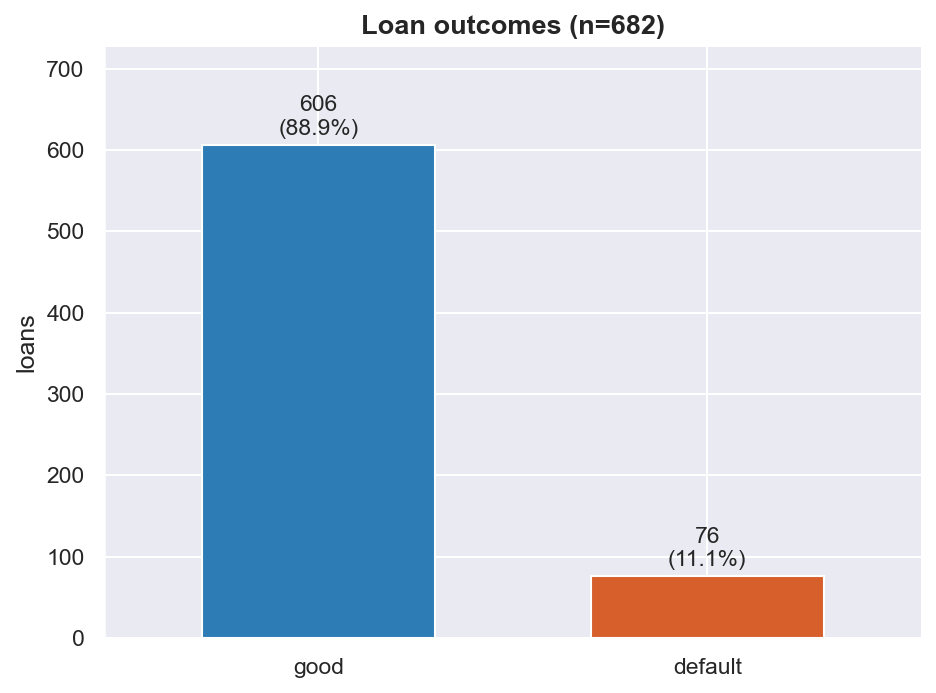
\includegraphics[width=0.9\textwidth]{figures/04_target_distribution.png}
    \caption{Target distribution: 606 good loans and 76 defaults}
    \label{fig:target_distribution}
\end{figure}

\section{Leakage Rule}
The defining constraint is that a feature may only use information available before the loan was granted. The feature query joins each loan to transactions with the condition \texttt{t.date\_id < l.loan\_date\_id}. Strict inequality matters: a transaction on the loan date is excluded. For each loan the aggregation computes transaction counts, turnover, average and standard deviation of amounts, average/minimum/maximum balance, the last balance before the loan, months active, and transaction frequency. All of these come from the pre-loan window.

The build performs an explicit audit: for each feature row it recounts the transactions that satisfy the date condition and compares that count with the stored \texttt{n\_txn}. A mismatch fails the build. The reported result is \texttt{features with post-loan rows: 0}, and the test suite checks the same condition. Figure~\ref{fig:feature_vector} shows how the source tables become one loan feature vector.

\begin{figure}[H]
    \centering
    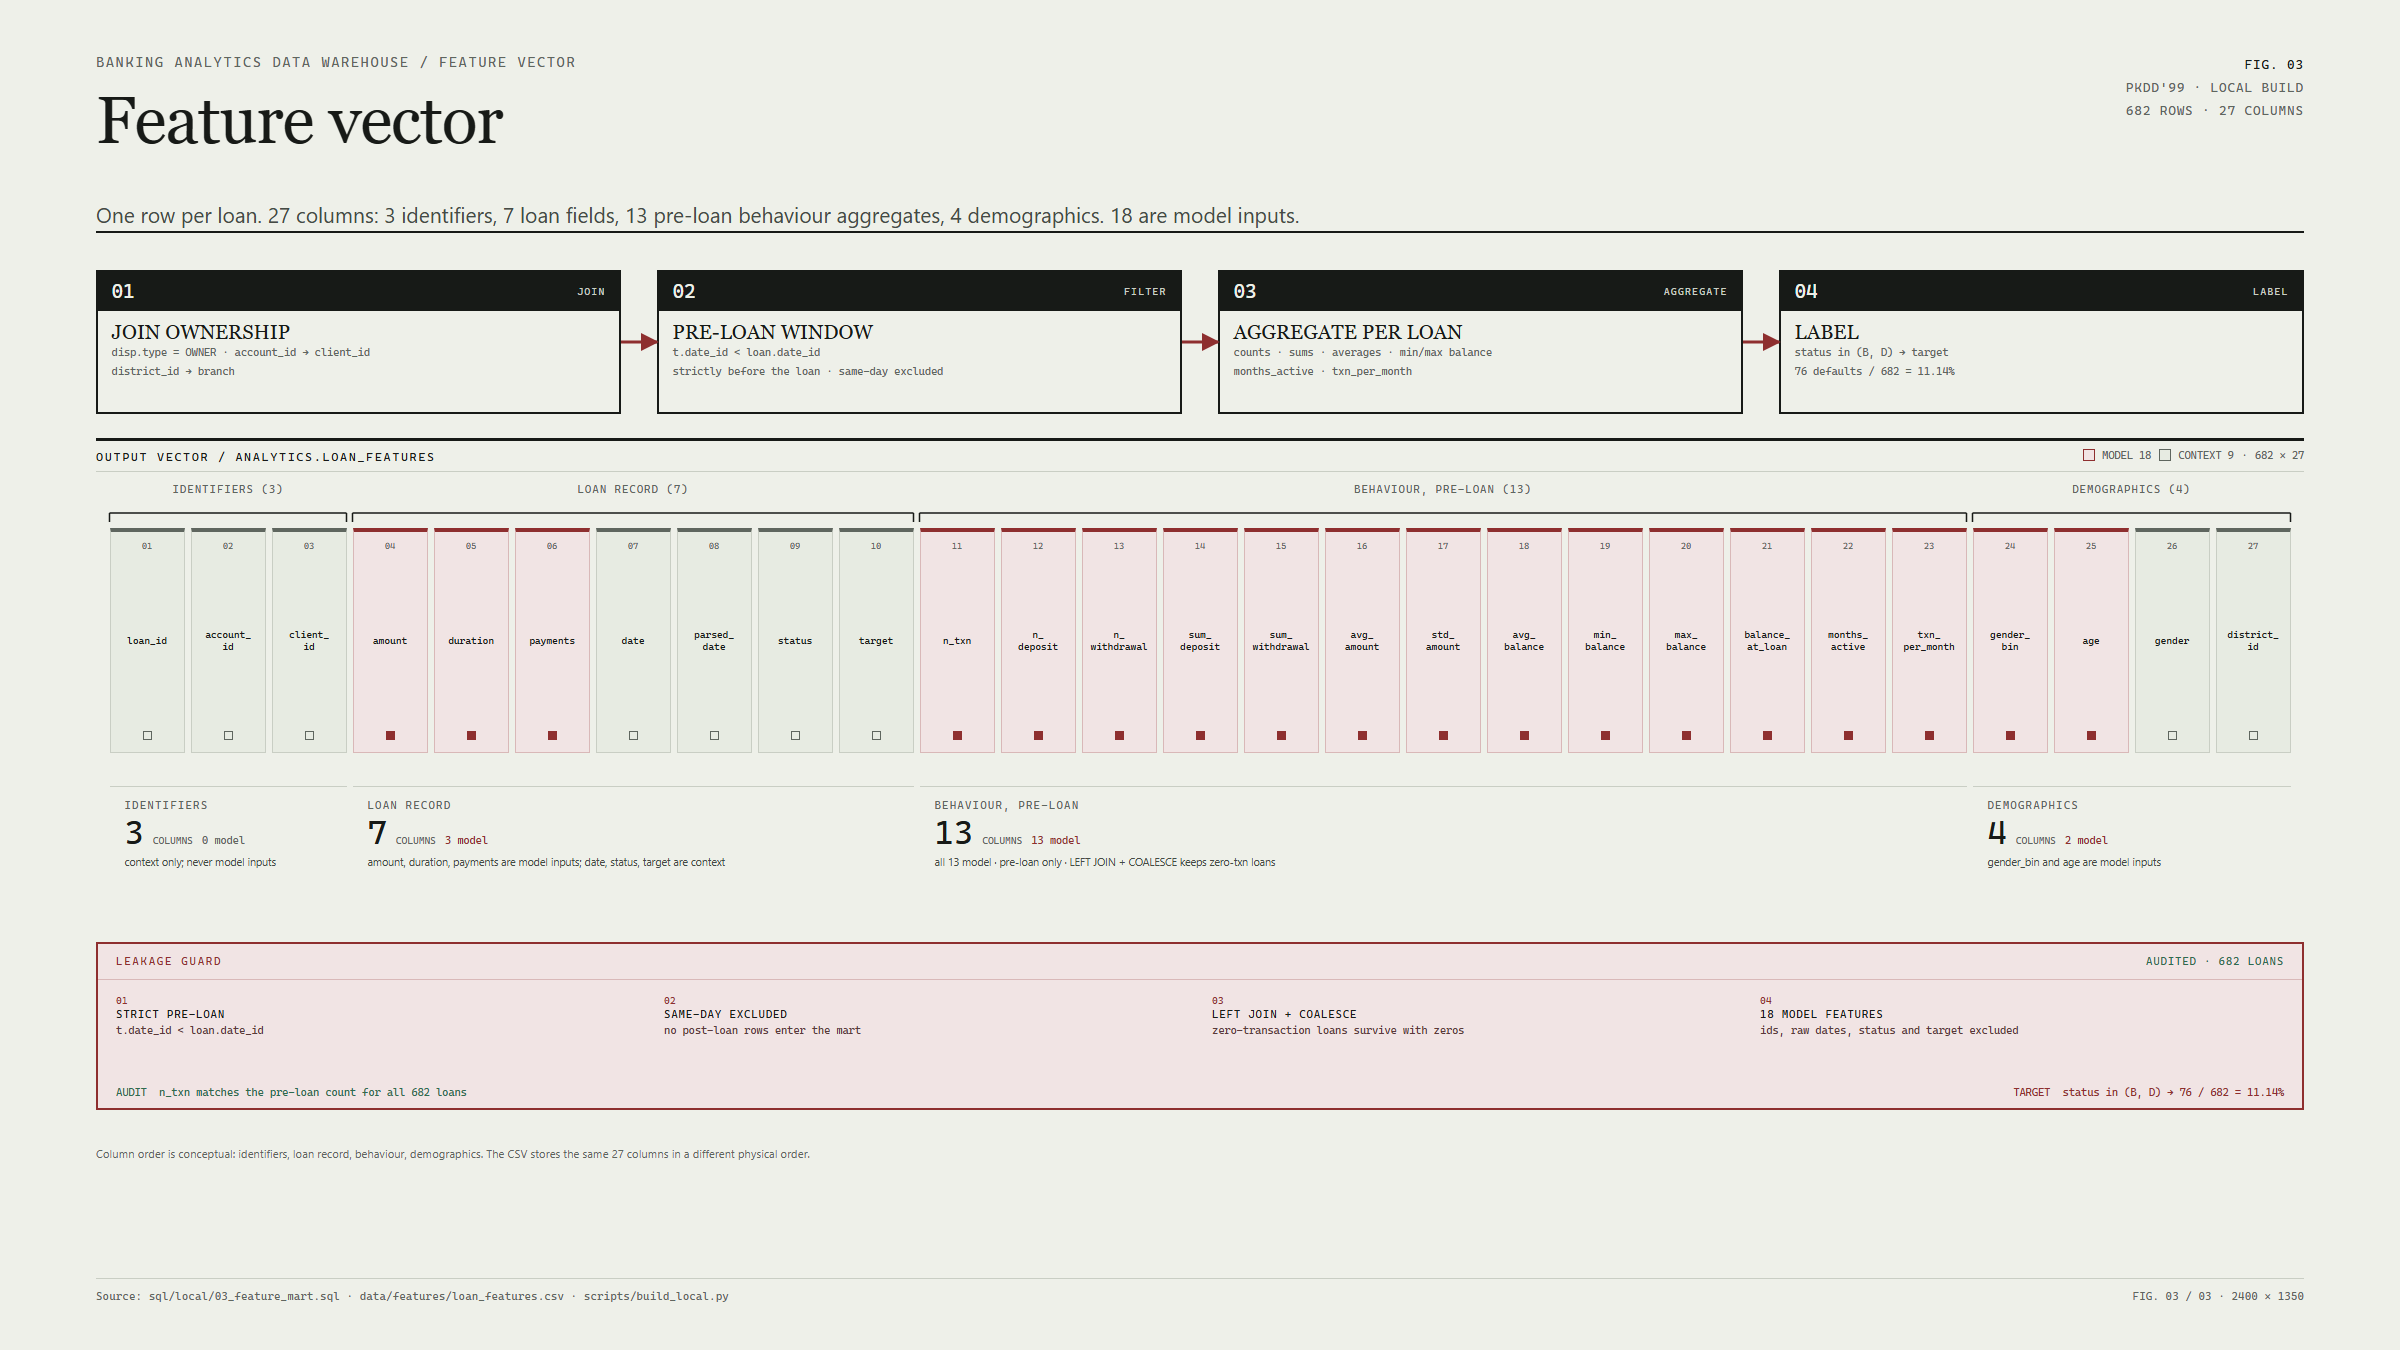
\includegraphics[width=0.9\textwidth]{figures/03_feature_vector.png}
    \caption{From source tables to a leakage-safe loan feature vector}
    \label{fig:feature_vector}
\end{figure}

\section{Feature Set}
Eighteen columns are used as model inputs. They fall into three groups:

\begin{table}[H]
    \centering
    \small
    \renewcommand{\arraystretch}{1.25}
    \begin{tabular}{|l|l|l|}
        \hline
        \textbf{Group} & \textbf{Count} & \textbf{Features} \\
        \hline
        Behavioural & 13 & \texttt{n\_txn}, \texttt{n\_deposit}, \texttt{n\_withdrawal}, \texttt{sum\_deposit}, \texttt{sum\_withdrawal}, \texttt{avg\_amount}, \texttt{std\_amount}, \texttt{avg\_balance}, \texttt{min\_balance}, \texttt{max\_balance}, \texttt{balance\_at\_loan}, \texttt{months\_active}, \texttt{txn\_per\_month} \\
        \hline
        Loan terms & 3 & \texttt{amount}, \texttt{duration}, \texttt{payments} \\
        \hline
        Demographics & 2 & \texttt{age}, \texttt{gender\_bin} \\
        \hline
    \end{tabular}
    \caption{The 18 modelling features}
    \label{tab:feature_groups}
\end{table}

Loan amount, duration, and payments describe the product; age and gender are limited demographics kept as a documented baseline. Behavioural features describe how the account was used before the loan. The unsupervised analysis in Chapter~9 deliberately drops the product and demographic columns and keeps only the 13 behavioural ones.

\section{Exploratory Findings}
The strongest correlations with default are negative balance measures: \texttt{min\_balance} ($-0.26$), \texttt{balance\_at\_loan} ($-0.20$), and \texttt{avg\_balance} ($-0.16$). Loan \texttt{payments} ($+0.18$) and \texttt{amount} ($+0.17$) are the next strongest. Median balance at the loan date is CZK 39,500 for good loans and CZK 22,000 for defaults, while transactions per month are nearly identical (5.7 versus 5.6).

A quadrant at the median balance and median loan amount makes the interaction clearer: the low-balance/high-amount group defaults at 23.3\%, against 4.9\% for high-balance/low-amount. A low balance combined with a large loan is the highest-risk combination, and this agrees with the feature importance reported in Chapter~8.

\section{Preprocessing Boundary}
Scaling, encoding, and oversampling are placed inside the fitted pipeline rather than applied to the whole table. The scaler is fitted on a training fold only, so validation and test folds are not contaminated by their own statistics. SMOTE, when used, is applied inside the training fold as well. This keeps the cross-validation comparison honest and is the second half of the project's leakage control.
